\documentclass[a4paper, 12pt]{article}
% math symbols
\usepackage{amssymb}
\usepackage{amsmath}
\usepackage{mathrsfs}
\usepackage{physsummer}


\usepackage{enumitem}
\usepackage[margin = 2cm]{geometry}

\tolerance = 1000
\emergencystretch = 0.74cm



\pagestyle{empty}
\parindent = 0mm

\begin{document}

\begin{center}
  \Large{\textbf{Городской центр физического образования, 10 класс.}\\
  \textit{Серия 17Ш, 2 марта 2015.}}
\end{center}

\begin{center}
  \Large\textbf{ Сложная электростатика. }
\end{center}

\Large

\task{ Два одинаковых проводящих шарика радиуса $R$ соединены тонкой
  натянутой проволочкой длины $L$ ($L \gg R$). Систему внесём в
  однородное электрическое поле $E_0$, направленное вдоль
  проволочки. Какой заряд протечёт по проволоке? Какое количества
  тепла выделится в сопротивлении проволоки? }
% Зильберман, ШФО, стр. 100

\task{ Плоский конденсатор состоит из двух больших пластин площадью
  $S$ каждая, расположенных на малом расстоянии $d$ ($S \gg d^2$) друг
  от друга. Пластины заряжены, их заряды $Q$ и $2Q$. Найдите разность
  потенциалов между пластинами. Пластины замыкают резистором
  $R$. Какой заряд протечёт по этому резистору? Сколько в нём
  выделится тепла? }
% Зильберман, ШФО, стр. 101

\taskpic{ Две материальные точки с массами $m$ и $M$ ($M>m$) и
  одинаковыми положительными зарядами $q$ находятся на расстоянии $l$
  друг от друга в однородном электрическом поле $E$, направленном от
  $m$ к $M$. В начальный момент скорости точек равны 0. Найдите
  максимальное расстояние между точками при их дальнейшем
  движении. Считайте, что точки всё время движутся вдоль одной
  прямой. }
{
  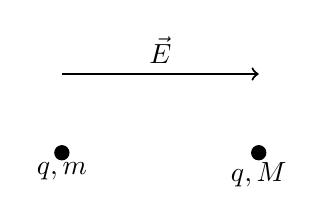
\begin{tikzpicture}
    \draw[fill=black] (0,0) circle (0.09cm) node[below] {$q,m$};
    \draw[fill=black] (2.5,0) circle (0.09cm) node[below] {$q,M$};
    \draw[thick,->] (0,1) -- (2.5,1) node[above,midway] {$\vec{E}$}; 
  \end{tikzpicture}
}
% Россия-2014, 10 класс

\task{ Проводящие сферы радиусов $R$ и $r$ находятся очень далеко друг
  от друга. Вначале они не заряжены. Батарейку напряжением $U_0$
  подключают очень тонкими проводами <<минусом>> к одной сфере и
  <<плюсом>> к другой. Найти заряд, протекший через батарею и работу
  батареи. Сравните эту работу с энергией получившегося поля. }
% Зильберман, ШФО, 5.21

\end{document}


%%% Local Variables: 
%%% mode: latex
%%% TeX-engine:xetex
%%% TeX-PDF-mode: t
%%% End:
